\chapter{Online planning}\label{chap:online planning}

\section{ Simulation }
The simulation is done online, but seeks to reduce the output to a minimum. The
main task is to visit all cells in the map and sweep them. This is simulated as
an online statemachine changing between different brahaviours of the robot.

\subsection{Behaviours}
There are basically three beahaviours of the robot:

\begin{itemize}
  \item Go to location
  \item Cover area
  \item Collect cup
\end{itemize}

The main task is solved using theese behaviours to visit all cells, covering the
cells, collecting the cups when inside range and returning the cups when ever
the tray is full.

\subsection{State machine}
The online simulation is done with a state machine facilitating the defined
behaviours. The state machine follows the diagram in figure
\ref{fig:statemachine}.

\begin{figure}[htb]
	\centering
	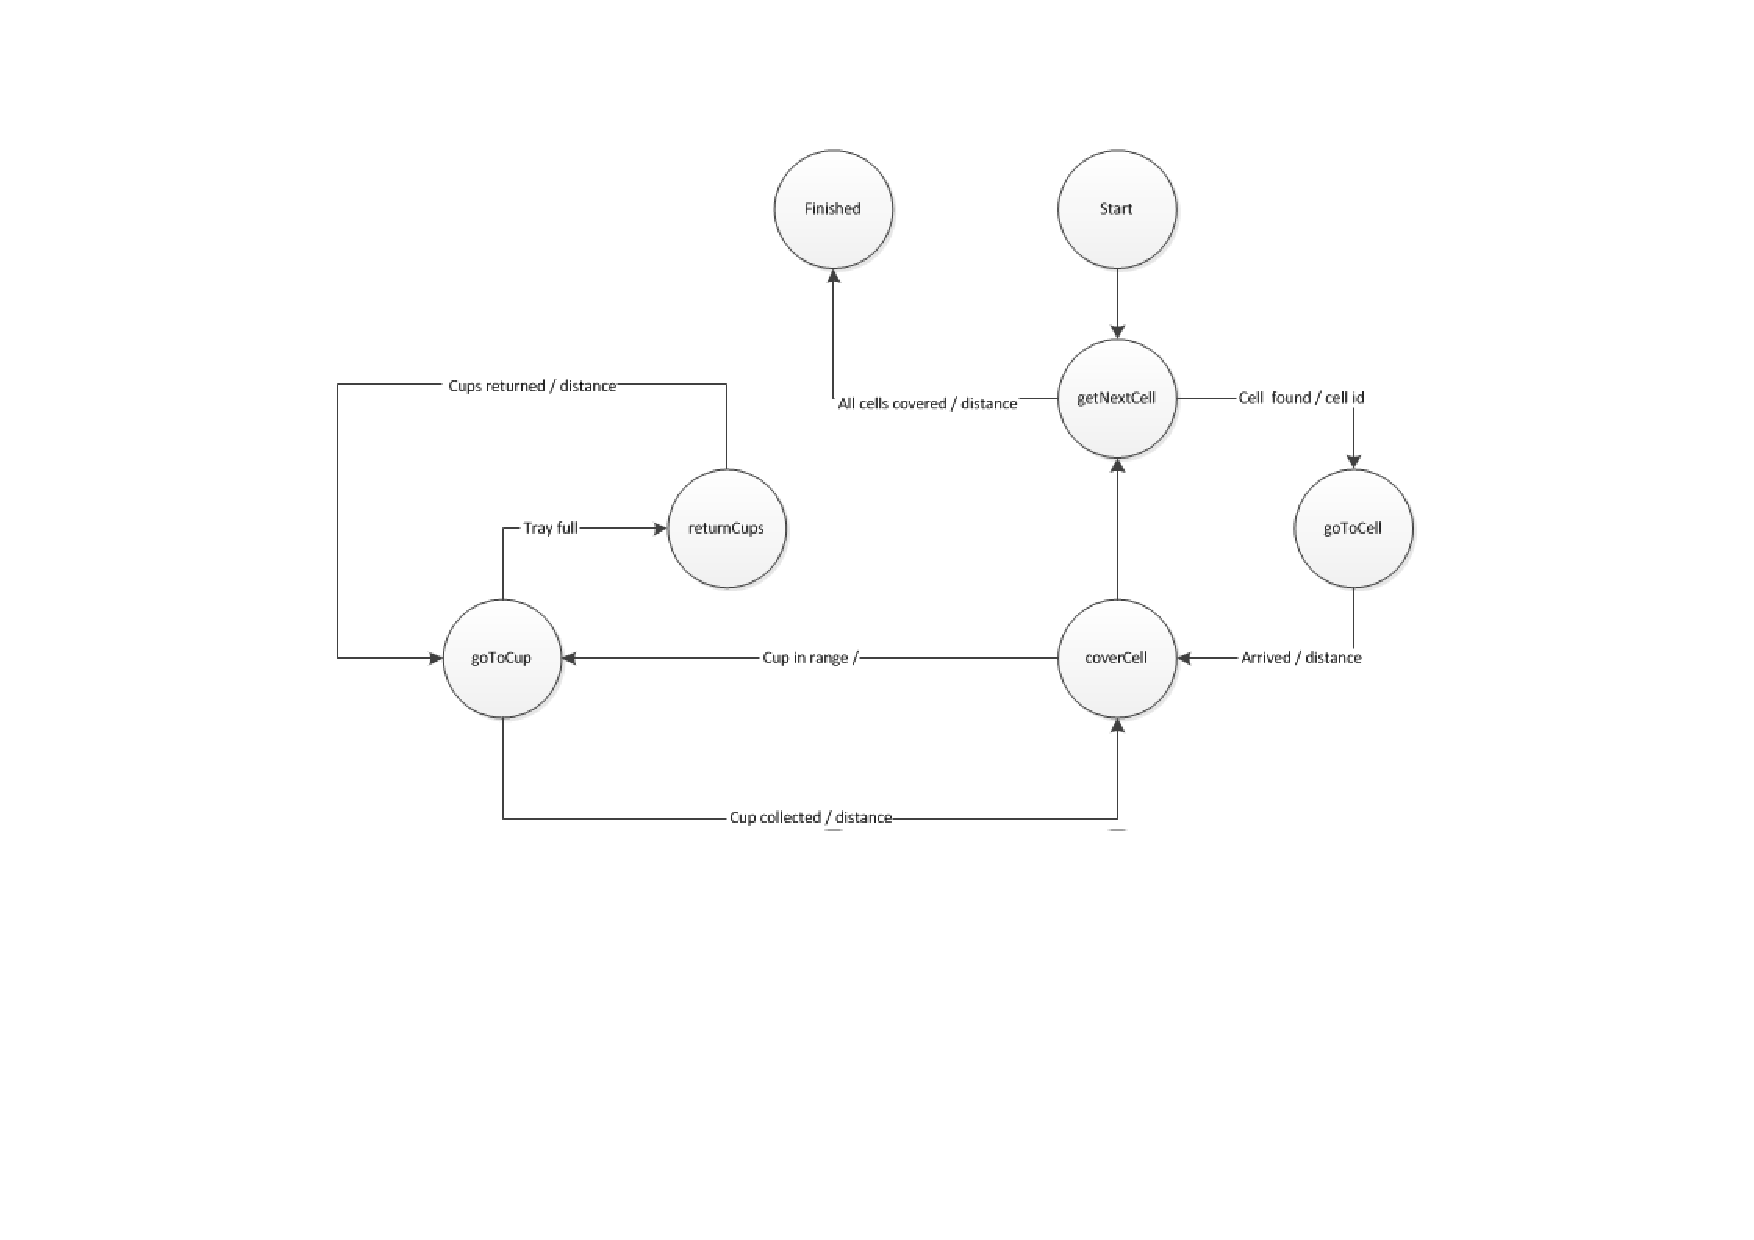
\includegraphics[width=\textwidth,trim=0 0 0 0]{graphics/statemachine.pdf}
	%trim=l b r t (can cut off from every side)
	\caption{State machine diagram}
	\label{fig:statemachine}			
\end{figure}